%As part of evaluation, we used rcu torture test. It provides support for testing all rcu implementations and gets enabled by config option CONFIG\_RCU\_TORTURE\_TEST. It creates an rcutorture kernel module that can be loaded to run torture test.  The test periodically outputs status messages via printk(), which can be examined via dmesg. The test gets started when the module is loaded, and stops when the module is unloaded. We verified our system by running it in a Guest virtual machine hosted by system equipped with an Intel(R) Core(TM) i7-860X 2.80 GHz CPUprocessor. In the course of evaluation all system was running Linux 2.6.32 kernel.
%As part of evaluation, we used microbenchmark and RCU torture test to determine the overhead posed by 
%\subsection{Hypothesis}
%Our evaluation strategy aims to test the following hypotheses:
Our evaluation strategy tests the following:
\begin{enumerate}
	\item[i)] Dynamic Binary Instrumentation (DBI) can be used to debug the incorrect usage of RCU primitives.
	\item[ii)] The performance overhead of Granary and Watchpoint used for debugging incorrect usage of RCU primitives.
	\item[iii)] The space overhead of shadow memory used for storing meta-information.
\end{enumerate}

\subsection{Performance Overhead}
\begin{figure}
\centering
 	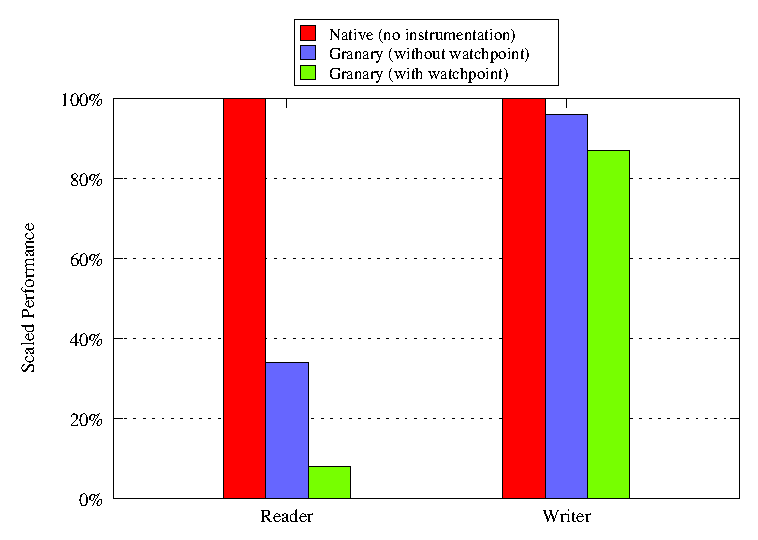
\includegraphics[width=0.45\textwidth]{performance}
\caption{Performance overhead for rcu torture test}\label{fig:perf}
\end{figure}
%We evaluated the performance of behavioural watchpoints using a microbenchmark and RCU torture test running with 100 readers and 5 writers. Our tests ran on a desktop equipped with an Intel\textregistered\ Core\texttrademark\ i7-860 2.80 GHz CPU, 8GB memory, and an Intel 82578DM Gigabit Ethernet card. Watchpoint instrumentation was enabled for every memory load and store, and watchpoints were active for all the RCU protected memory allocated from the memory pool.
We evaluated the performance of behavioural watchpoints using a microbenchmark and RCU torture. Our tests ran on a desktop equipped with an Intel\textregistered\ Core\texttrademark\ i7-860 2.80 GHz CPU, 8GB memory, and an Intel 82578DM Gigabit Ethernet card. Watchpoint instrumentation was enabled for every memory load and store, and watchpoints were active for all the RCU protected memory allocated from the memory pool.

\paragraph{Microbenchmark} The microbenchmark performed a tight-loop of memory operations on watched addresses and exhibits the worst-case performance overhead of watchpoints (about 20{\footnotesize$\times$}). This is expected because our instrumentation adds instructions to each memory load and store.
 %added to all memory returned from kernel heap allocators. 
%To evaluate the performance overhead incurred by the Granary and watchpoint we used rcutorture module running with 100 reader and 5 writer threads. As experimental setup, we run our system in Guest Virtual machine (QEMU) running with four core and powered with Linux 2.6.32 kernel on a Host system equipped with an Intel(R) Core(TM) i7-860, 2.80 GHz CPU. Our evaluation strategy involves running rcutorture module natively, under the control of Granary \& Granary with watchpoint active and studying the following parameters :
%\paragraph{\texttt{rcutorture}} We tested the \texttt{rcutorture} kernel module. It exhibited interesting behaviour: all threads experienced a minimum of 6{\footnotesize$\times$} overhead; however, readers were abnormally penalized and tended to see more stale data. We think this is because each writer synchronized with fewer readers.
%\paragraph{RCU tortute test} We tested the performance overhead incurred by Granary and watchpoints using \texttt{rcutorture} kernel module. Our evaluation strategy involves running rcutorture module natively, under the control of Granary \& Granary with active watchpoints and studying the following parameters :
\paragraph{RCU torture test} RCU torture is a kernel module which tests the
performance and correctness of RCU. We used this module to test the
performance overhead of Granary and watchpoints. The module was setup to
run with 5 updaters and a 100 readers. It was run
natively, under the control of Granary \& finally under
Granary with active watchpoints. We observed the following:
\begin{enumerate}
	\item[i)] The number of successful updates
	\item[ii)] The number of successful reads/
\end{enumerate}
%We recorded these parameters by running rcutorture module for 60 sec and averaged it over five different runs. Table~\ref{table:nonlin} below shows these parameters for three different cases. Our experimental result shows moderate decrease in ver number which shows the number of times writer task has changed the structure visible to readers but there is a drastic decrease in the readers \emph{Readers Pipe} and \emph{Readers batch} showing the increase in the readers seeing stale data. We think this is because each writer synchronized with fewer readers. The performance of readers and writers based on these parameters is shown in figure~\ref{fig:perf}.
We recorded these parameters by running rcutorture module for 60 sec and
averaged it over five different runs. Figure~\ref{fig:perf} shows the
results obtained. As can be seen, there is moderate decrease in the number
of updates and a drastic decrease in number of readers. This is because
where there was minimal overhead on the read critical section, we have
added additional instructions to instrument RCU.



% The result shows a moderate decrease in the performance of writer but the performance of readers decreases by approximately 10 times. One of the reason for this is we are testing the system with 100 readers but only 5 writers thread and read is the most frequent operation in the rcu torture test. Our system also instrument both memory read and write which is going to be costly but it gets amortized over the large number of instructions.

%\begin{table*}[thp!]
%\caption{Reader and Writer performance for rcu torture test}
% title of Table
%\centering
% used for centering table
%\begin{tabular}{c c c c}
% centered columns (4 columns)
%\hline\hline
%inserts double horizontal lines
%rcu-tortute-test & Ver & Reader-Pipe & Reader-Batch  \\ [0.5ex]
% inserts table
%heading
%\hline
% inserts single horizontal line
%Native(no instrumentation) & 2112 & 233093662 & 214069371 \\
% inserting body of the table
%Granary(without watchpoint) & 2043 & 87237464 & 83627748 \\
%Granary(with watchpoint) & 1850 & 16996975 & 16996075 \\[1ex]
% [1ex] adds vertical space
%\hline
%inserts single line
%\end{tabular}
%\label{table:nonlin}
% is used to refer this table in the text
%\end{table*}

%The other interesting observation we made is decrease in the performance overhead is not much because of watchpoint. There is significant drop in the performance of readers when rcutorture is run under the control of granary and watchpoint is not active. One reason for this is we annotated all rcu read side primitive to make a callback to kernel wrapper. These kernel wrapper runs natively and are not in code-cache. There is a cost involved when Granary switches execution from the code-cache to native since it has to switch the stack and save and restore the machine context. We have seen similar behaviour earlier with other file-system modules while running benchmarks like postmark~\cite{katcher97postmark} which involves many context switches. We have not yet verified this with rcutorture module.

The more interesting observation is that the decrease in performance
overhead is mainly caused due to Granary and not watchpoint. The
primary reason for this is that the rcu read critical section primitives
were annotated to make a callback into the wrapper. The kernel wrapper
runs natively and is not present in the code-cache. Switching execution
from code-cache to native has a performance impact since Granary has
to switch the stack, and save and restore the machine context. We have
seen similar behavior with file-system modules running other benchmarks
which involved many context switches. We are still to verify these
with RCU torture.

\subsection {RCU debugger}
To evaluate our system for rcu debugging, we introduced few rcu bugs violating
Rule 0, 1 and 2, as discussed in section ~\ref{sec:back}. Some examples of
these bugs are shown in Figures\textbf{AKSHAYTHEREISNORCUuseRule0figure}~\ref{RCUuseRule0},~\ref{fig:rcuderefbug} and~\ref{fig:rcuusebug}.
The first bug violated Rule 0 where the alias \emph{p} of RCU protected
date \emph{q} is referenced outside the read critical section. We
identify it by comparing the \emph{generation number} and watchpoint
\emph{generation number}. We find that the thread \emph{generation number}
is odd and not equal to the watchpoint \emph{generation number} at the
point of memory reference. The second bug we introduced violated Rule 1.
The RCU protected data \emph{q} was directly accessed without using
\emph{rcu\_dereference}. We notice at the time of access that the pointer
is a source and not an alias generated by \emph{rcu\_dereference}. This
is done by by checking \emph{meta\_info$\rightarrow$source}. We also notice
at this point that the \emph{generation number} and watchpoint \emph{generation number}
are not the same. We tesed Rule 3 violation by dereferencing RCU pointer in
a read critical section other than where it was aliased using \emph{rcu\_dereference}.
We tested this for a simple case where there is no recursive use of read critical
section. We identify this by checking both thread as well as generation
\emph{generation numbers}.

%To evaluate our system for rcu debugging, we introduced few rcu bugs violating Rule 0, 1 and 2, as discussed in section ~\ref{sec:back}. The details of the introduced bugs is provided in figure~\ref{fig:RCUuseRule0},~\ref{fig:rcuderefbug} and~\ref{fig:rcuusebug}. The first bug voilate Rule 0 where the alias \emph{p} of rcu protected data \emph{q} is getting referenced outside read critical section. Our system identified it by comparing the thread \emph{generation number} and watchpoint \emph{generation number}. Our system found the thread \emph{generation number} is odd and not equal to watchpoint \emph{generation number} at the point of memory reference. The second bug we introduced voilates Rule 1, where the rcu protected data \emph{q} is directly getting accessed without using \emph{rcu\_dereference()}. Our system noticed that when the memory gets accessed, the pointer is a source and not one of  alias generated by \emph{rcu\_dereference()} by checking \emph{meta\_info$\rightarrow$source}. Our system also noticed that at this point the thread \emph{generation number} and watchpoint \emph{generation number} is not same. We also tested the Rule 3 violation by dereferncing rcu pointer in read critical section other than the one where it gets alias using \emph{rcu\_dereference()}. We tested this for simple case where there is no recursive use of read critical section. Our system identifies this by checking both thread \emph{generation number} and watchpoint \emph{generation number}. 

%We evaluated our system by introducing simple bugs in rcutorture module and found that it catches the violation of three rules mentioned in section~\ref{sec:back}. There is need to test the system with complex rcu bugs which includes the voilation of more than one rules and corner cases. We are hopeful that our system will be able to catch such bugs also.

We evaluated our system by introducing simple bugs in rcutorture module and
found that it detects the violation of three rules mentioned in
section~\ref{sec:back}. There is need to test the system with complex rcu bugs
which violate multple rules and corner cases. We expect
that our system will be able to catch most of these bugs.


\subsection{Space Overhead}
The size of shadow memory depends on the number of watchpoints added and currently active. Shadow memory is used to store the meta-information, the size of which is proportional to the number of threads running. This increases the space overhead and makes it \emph{M x N} for the system running \emph{N} threads and having \emph{M} active watchpoint. The point to be noted that this is the virtual memory overhead. We do not expect the space overhead to be serious concern on a 64 bit architecture.    


